\chapter{Results}\label{chap:results}
\begin{overview}
  Results of the techniques whose implementation was discussed in the
  previous part are shown here.  The result of various event
  identification techniques are shown, followed by examples of models
  built using the Modelica package and the results of the simulation of these models.
\end{overview}

\section{Event identification}
\subsection{Test signals}
To illustrate the type of result that is obtained using the technique,
we show the results on a a signal consisting of 6 events, attempting
to fit 4 events.  Figure~\ref{fig:front_evolution} shows the evolution
of the Pareto front in terms of fit complexity and RMS error for
different numbers of iterations.

\begin{figure}[htbp]
  \centering
  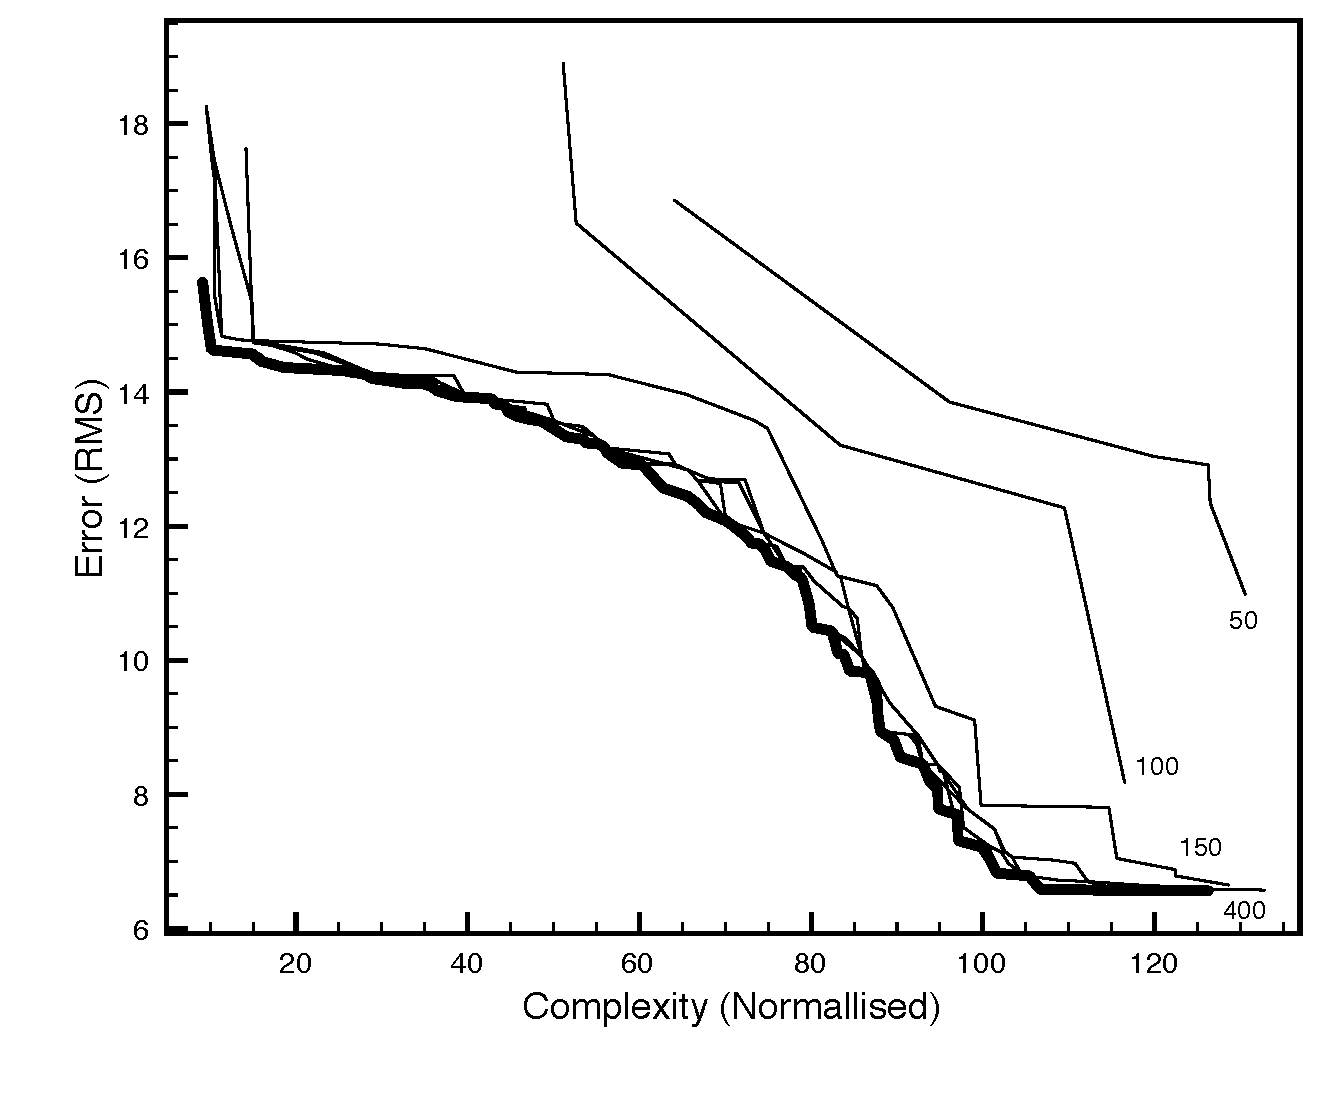
\includegraphics[width=0.7\textwidth]{front_evolution}
  \caption{Evolution of Pareto Front for 6 events being fit by 4 events.}
  \label{fig:front_evolution}
\end{figure}

It should be noted that, although the front seems to be converging,
population based multi-objective optimisation algorithms can not
guarantee convergence with a finite archive.  This is due to the
pruning that must inevitably be done when the archive is full.
Figure~\ref{fig:front_evolution} does, however, show that the front has not
receded.

\subsection{Real-life signals}


\section{Models}

\section{Simulation results}


% Local Variables:
% TeX-master: "thesis"
% End:
